\documentclass[a4paper]{article}

\input{style/ch_xelatex.tex}
\input{style/scala.tex}

\usepackage[fontset=none]{ctex}
\usepackage{graphicx}
\usepackage{color,framed}
\usepackage{listings}
\usepackage{caption}
\usepackage{amssymb}
\usepackage{enumerate}
\usepackage{xcolor}
\usepackage{bm}
\usepackage{lastpage}
\usepackage{fancyhdr}
\usepackage{tabularx}
\usepackage{geometry}
\usepackage{graphics}
\usepackage{subfigure}
\usepackage{float}
\usepackage{pdfpages}
\usepackage{pgfplots}
\usepackage{multirow}
\usepackage{footnote}
\usepackage{booktabs}
\usepackage{hyperref}

\setmainfont{Times New Roman}
\setsansfont{Arial}
\setmonofont{Menlo}
\setCJKmainfont{STSong}
\setCJKsansfont{Heiti SC}
\setCJKmonofont{STSong}
\allsectionsfont{\sffamily}

\pgfplotsset{width=10cm,compat=1.9}

\lstset{
breaklines=true,
basicstyle=\small\ttfamily,
keywordstyle=\color{blue!70}\bfseries,
commentstyle=\color{red!50!green!50!blue!50},
stringstyle=\ttfamily,
extendedchars=false,
linewidth=\textwidth,
numbers=left,
numberstyle=\tiny \color{blue!50},
frame=trbl,
rulesepcolor=\color{red!20!green!20!blue!20}
}

\geometry{a4paper,left=2.3cm,right=2.3cm,top=2.7cm,bottom=2.7cm}
\pagestyle{fancy}
\lhead{\leftmark}
\rhead{PA3 实验报告}
\lfoot{}
\cfoot{\thepage}
\rfoot{}
\renewcommand{\headrulewidth}{0.1pt}
\renewcommand{\footrulewidth}{0pt}
\setlength{\textfloatsep}{8mm}
\graphicspath{{images/}{fig/}}

\begin{document}
\renewcommand{\contentsname}{目\ 录}
\renewcommand{\appendixname}{附录}
\renewcommand{\appendixpagename}{附录}
\renewcommand{\refname}{参考文献}
\renewcommand{\figurename}{图}
\renewcommand{\tablename}{表}
\renewcommand{\today}{\number\year 年 \number\month 月 \number\day 日}

\begin{titlepage}
  \begin{center}
    
\includegraphics[width=0.8\textwidth]{NKU.png}\\[1cm]
    \vspace{18mm}
    \textbf{\huge\textbf{计算机学院}}\\[0.5cm]
    \textbf{\huge{计算机系统基础（PA）实验报告}}\\[2.1cm]
    \textbf{\Huge\textbf{PA3：异常控制流与操作系统}}

    \vspace{\fill}
    \centering
    \textsc{\LARGE 姓名\ :\ 林晖鹏}\\[0.5cm]
    \textsc{\LARGE 学号\ :\ 2312966}\\[0.5cm]
    \textsc{\LARGE 专业\ :\ 计算机科学与技术}\\[0.5cm]

    \vfill
    {\Large \today}
  \end{center}
\end{titlepage}

\renewcommand{\thefigure}{\thesection{}.\arabic{figure}}
\renewcommand{\contentsname}{目录}
\cfoot{\thepage\ of \pageref{LastPage}}

\clearpage
\tableofcontents
\newpage

\section{概述}
PA3 对整个工程的要求比前两个阶段明显更高。NEMU 不再只需要支撑裸机上的 AM 程序，系统还要继续向上承载一个最小操作系统 Nanos-lite，再由 Nanos-lite 去装载和执行用户程序。实验做到这里，关注点已经从补齐单条指令，逐渐转到把 \texttt{NEMU}、\texttt{AM}、\texttt{Nanos-lite}、\texttt{Navy-apps} 四层接成一条能运行的链路。

从系统结构上看，PA3 主要完成了三件事。第一，把 \texttt{dummy}、\texttt{hello} 等用户程序打包进 \texttt{ramdisk} 并由 \texttt{loader()} 装载执行；第二，在 NEMU 中加入 \texttt{IDTR}、\texttt{lidt}、\texttt{int}、\texttt{iret}、\texttt{pusha}、\texttt{popa} 等异常控制流相关能力，使系统调用能够从用户态陷入内核，再从内核正确返回；第三，在 Nanos-lite 中补齐最小系统调用、简易文件系统和设备文件接口，让 \texttt{hello}、\texttt{text}、\texttt{bmptest}、\texttt{pal} 等程序最终能够运行。

\section{实验目的}
本次实验的目标，不只是把某个程序跑起来，而是理解操作系统这一层到底给程序补上了什么。具体来说，这里希望通过 PA3 弄清楚三件事：第一，用户程序是如何从 \texttt{navy-apps} 被编译、打包进 \texttt{ramdisk}，再由 Nanos-lite 装载执行的；第二，i386 异常控制流的最小工作机制是什么，系统调用又是如何借助 \texttt{IDT}、\texttt{IDTR}、\texttt{lidt}、\texttt{int}、\texttt{iret} 和 trap frame 从用户态陷入内核并返回的；第三，操作系统怎样通过文件系统和设备文件向用户程序提供统一接口。最终的验收目标则是让 \texttt{hello}、\texttt{text}、\texttt{bmptest} 以及 \texttt{pal} 都真正运行起来。

\section{实验内容}
结合指导书和实际实现过程，这里把 PA3 的内容分成了三条连续主线。第一条主线是装载第一个用户程序，也就是确认 \texttt{loader()} 已经能够把 \texttt{dummy} 从 \texttt{ramdisk} 搬到固定入口地址并开始执行；第二条主线是加入 ASYE 支持，打通 \texttt{int \$0x80} 到 \texttt{do\_syscall()} 再到 \texttt{iret} 的异常控制流与系统调用最小闭环；第三条主线则是把内核真正做成一个可用的最小操作系统，补齐 \texttt{SYS\_write}、\texttt{SYS\_brk}、简易文件系统以及 \texttt{/dev/fb}、\texttt{/proc/dispinfo}、\texttt{/dev/events} 等设备文件接口，最后去支撑完整用户程序运行。

\section{加载第一个用户程序并验证 raw loader}

\subsection{编译并打包第一个用户程序}
PA3 的第一步是先得到一个真正运行在 Nanos-lite 之上的用户程序。本次选择的第一个目标程序是 \texttt{navy-apps/tests/dummy/dummy.c}。

最开始在 \texttt{navy-apps/tests/dummy} 下直接执行 \texttt{make}，结果构建系统尝试生成的是 \texttt{dummy-native}，并在链接阶段报出 \texttt{undefined reference to '\_syscall\_'}。这说明当时程序被编译到了宿主机的 \texttt{native} 目标，而不是 PA3 所要求的 x86 用户程序目标。之后改为显式指定：
\begin{lstlisting}[language=bash]
make ISA=x86
\end{lstlisting}
运行结果中可以看到生成了 \texttt{dummy-x86}。此时得到的二进制才是后续由 Nanos-lite 装载的真实用户程序。

接下来需要在 \texttt{nanos-lite} 目录下执行：
\begin{lstlisting}[language=bash]
make update
\end{lstlisting}
这一步会将刚刚构建好的 \texttt{dummy-x86} 通过 \texttt{objcopy} 抽取成裸二进制，并写入 \texttt{build/ramdisk.img}。这也是为什么在 PA3 中每当用户程序发生变化后，都必须重新执行一次 \texttt{make update}，否则 \texttt{loader()} 读到的仍然会是旧版本程序。

\subsection{实现最小化 raw loader}
这一阶段的用户程序装载逻辑非常简单，因为 \texttt{ramdisk} 中只有一个用户程序，而且指导书已经约定：用户程序入口固定为 \texttt{0x4000000}，同时程序内容从 \texttt{ramdisk} 偏移 \texttt{0} 开始存放。也就是说，这里不需要文件系统，不需要按名字找文件，更不需要 ELF 解析，只要把这一整段内容搬到约定入口即可。

因此，\texttt{loader()} 的最小实现其实就是一个很短的动作链：先调用 \texttt{get\_ramdisk\_size()} 拿到程序大小，再通过 \texttt{ramdisk\_read(DEFAULT\_ENTRY, 0, size)} 把整段二进制复制到 \texttt{0x4000000}，最后把这个入口地址返回给上层。

真正落代码时，这里还是把它拆得更细一些：先在 \texttt{loader.c} 中把 \texttt{ramdisk\_read()} 和 \texttt{get\_ramdisk\_size()} 接进来，再定义固定入口 \texttt{DEFAULT\_ENTRY = 0x4000000}，然后在 \texttt{loader()} 里先求完整长度、再复制整段程序、最后把入口返回给调用者。这样虽然实现很短，但逻辑上是完整的。

这样写的好处是逻辑非常直接：当前阶段不需要考虑文件名、偏移表、ELF 头或段映射，先确认用户程序已经能够被装入并开始执行。

本次在 \texttt{nanos-lite/src/loader.c} 中补上的核心代码如下：
\begin{lstlisting}[language=C]
#define DEFAULT_ENTRY ((void *)0x4000000)

uintptr_t loader(_Protect *as, const char *filename) {
  ramdisk_read(DEFAULT_ENTRY, 0, get_ramdisk_size());
  return (uintptr_t)DEFAULT_ENTRY;
}
\end{lstlisting}

这段代码虽然短，但每一行都对应了一个明确动作。第一行先定义固定入口地址 \texttt{DEFAULT\_ENTRY}，表示当前阶段用户程序的装载位置；\texttt{loader()} 的第一句通过 \texttt{get\_ramdisk\_size()} 隐式确定了需要搬运的数据总长度；随后 \texttt{ramdisk\_read(DEFAULT\_ENTRY, 0, size)} 把 \texttt{ramdisk} 中从偏移 \texttt{0} 开始的整段用户程序复制到内存入口处；最后返回这个入口地址，供上层后续跳转使用。

这里没有继续往前引入文件系统或 ELF 解析，而是先保留最短装载路径。这样做之后，运行时一旦继续向前推进到 \texttt{int 0x80}、\texttt{invalid opcode} 等位置，就可以确认用户代码本身已经被装入并开始执行，后续排查的重点也能稳定落到异常机制上。

\subsection{运行现象与阶段结论}
在 \texttt{nanos-lite} 目录下执行：
\begin{lstlisting}[language=bash]
make ARCH=x86-nemu run
\end{lstlisting}
进入 NEMU monitor 后再输入 \texttt{c} 继续执行，最终看到用户程序停在未实现的 \texttt{int 0x80} 处。对应截图如图 \ref{fig:pa3-loader-int80} 所示。

\begin{figure}[H]
  \centering
  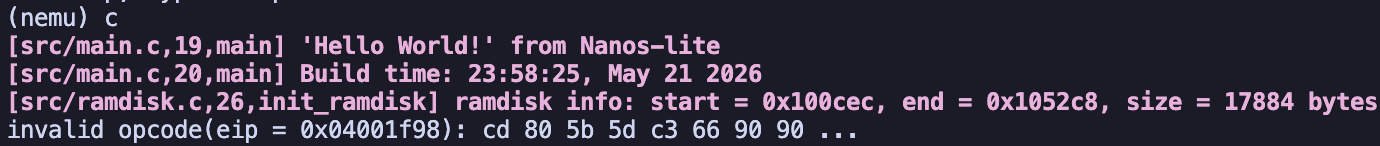
\includegraphics[width=0.82\textwidth]{pa3-loader-int80.png}
  \caption{raw loader 已经成功把 \texttt{dummy} 装入内存，并推进到 \texttt{int 0x80}}
  \label{fig:pa3-loader-int80}
\end{figure}

运行停在这里之后，定位就清楚了：用户程序装载已经没有问题，后续阻塞点集中在异常与系统调用机制本身。到这一步为止，\texttt{loader()} 的阶段任务已经完成，后面的修改重点自然转到 ASYE 和系统调用链路上。

\section{异常控制流、trap frame 与系统调用最小闭环}

\subsection{加入 ASYE 的最小骨架}
为了让 \texttt{int \$0x80} 不再被 NEMU 当作普通非法指令，必须先把异常控制流的硬件侧和 AM 侧骨架接起来。这里的改动主要集中在六个点上：给 \texttt{CPU\_state} 增加 \texttt{IDTR} 和 \texttt{CS}，实现 \texttt{lidt}，在 \texttt{restart()} 中补上 \texttt{CS=0x8} 和 \texttt{EFLAGS=0x2} 的初始化，在 \texttt{nanos-lite/src/main.c} 中打开 \texttt{HAS\_ASYE}，再在 NEMU 中实现 \texttt{int}、\texttt{raise\_intr()} 和 \texttt{iret}。这样一来，异常机制的入口、现场保存和返回路径才都具备了。

\texttt{raise\_intr()} 的简化实现思路与 i386 手册中的最小过程一致：压入 \texttt{EFLAGS}、\texttt{CS} 和返回地址，再根据 \texttt{IDTR} 和异常号定位门描述符，最后把 \texttt{EIP} 切换到异常入口。这样做的好处是：后面无论是软件异常还是硬件中断，都可以复用同一条入口逻辑。

这一部分在代码实现时，实际是按先让表能装进去、再让异常能跳进去、最后再让它能退出来的顺序推进的。也就是说，先补 \texttt{IDTR/CS} 和 \texttt{lidt}，再让 \texttt{int} 统一走 \texttt{raise\_intr()}，最后才补 \texttt{iret}。这样每往前走一步，运行时的阻塞点都会推进到下一处，而不是一上来改很多地方却不知道到底是谁起了作用。

这里除了写 helper 本身，还必须把这些指令真正接进 opcode table。当前工程里对应的接线是：
\begin{lstlisting}[language=C]
/* 0x60 */ EX(pusha), EX(popa), EMPTY, EMPTY,
...
/* 0xcc */ EMPTY, IDEXW(I, int, 1), EMPTY, EX(iret),
\end{lstlisting}

而 \texttt{lidt} 则是挂在两字节转义指令组里：
\begin{lstlisting}[language=C]
make_group(gp7,
    EMPTY, EMPTY, EMPTY, EX(lidt),
    EMPTY, EMPTY, EMPTY, EMPTY)
\end{lstlisting}

这几行代码在实现过程中其实非常关键。比如 \texttt{int} helper 就算已经写好，如果 \texttt{0xcd} 这个 opcode 没有在表里接到 \texttt{IDEXW(I, int, 1)}，运行时仍然只会停在原地报未实现指令；\texttt{iret} 也是同样的道理。也就是说，NEMU 里一条指令要真正可用，不仅要 helper 语义正确，还必须在 opcode table 中能被正确分发到。

其中 \texttt{raise\_intr()} 的核心代码结构如下：
\begin{lstlisting}[language=C]
void raise_intr(uint8_t NO, vaddr_t ret_addr) {
  rtl_push(&cpu.eflags.val);
  rtl_push(&cpu.cs.val);
  rtl_push(&ret_addr);
  cpu.cs.val = 0x8;

  GateDesc gate;
  vaddr_t addr = cpu.idtr.base + NO * sizeof(GateDesc);
  gate.val[0] = vaddr_read(addr, 4);
  gate.val[1] = vaddr_read(addr + 4, 4);

  cpu.eip = gate.offset_15_0 | (gate.offset_31_16 << 16);
}
\end{lstlisting}

这段代码可以按保存旧现场和找到新入口两个部分来理解。前三个 \texttt{rtl\_push()} 依次把 \texttt{EFLAGS}、\texttt{CS} 和返回地址压栈，相当于为未来的 \texttt{iret} 提前保存恢复所需的信息；接着把 \texttt{cpu.cs.val} 设成 \texttt{0x8}，表示后续开始按照内核代码段执行。下面一段通过 \texttt{cpu.idtr.base + NO * sizeof(GateDesc)} 计算 IDT 中对应门描述符的位置，再把门描述符里的高低位偏移拼成新的 \texttt{EIP}，于是控制流就真正跳到了异常入口。

系统调用和中断都不是普通函数调用。普通函数主要依赖返回地址继续执行，异常控制流还要把标志寄存器和代码段一起保留下来，否则回到用户态时现场无法恢复。PA3 里的 \texttt{int \$0x80}、\texttt{SYS\_write}，以及后面 PA4 的时钟中断，实际都沿着这条统一入口路径工作。

\texttt{lidt}、\texttt{int} 和 \texttt{iret} 本身在代码里也各自补了最小语义。例如 \texttt{system.c} 里的 \texttt{int} 和 \texttt{iret} 实现如下：
\begin{lstlisting}[language=C]
make_EHelper(int) {
  raise_intr(id_dest->val, decoding.seq_eip);
}

make_EHelper(iret) {
  rtl_pop(&decoding.jmp_eip);
  rtl_pop(&t0);
  cpu.cs = (uint16_t)t0;
  rtl_pop(&t1);
  cpu.eflags = t1;
  decoding.is_jmp = 1;
}
\end{lstlisting}

\texttt{int} 这里做的事情很集中，就是把异常号和“下一条指令地址”交给 \texttt{raise\_intr()}。之所以传 \texttt{decoding.seq\_eip}，是因为将来从 \texttt{iret} 返回时，系统应该继续执行 \texttt{int \$0x80} 后面的那条指令。下面的 \texttt{iret} 则完全对应 i386 的返回语义：按相反顺序把之前压入栈中的 \texttt{EIP}、\texttt{CS} 和 \texttt{EFLAGS} 取回来，最后把 \texttt{decoding.is\_jmp} 置 1，告诉执行框架后续应该从新的 \texttt{EIP} 继续。

\subsection{从 \texttt{lidt} 到 \texttt{vecsys()} 的逐步推进}
这一阶段的调试过程更适合按阻塞点如何向前推进来记录。最开始打开 \texttt{HAS\_ASYE} 之后，程序已经不再直接停在用户程序中的 \texttt{cd 80}，而是继续执行到 \texttt{init\_irq()} 和 \texttt{\_asye\_init()} 附近，然后在 \texttt{lidt} 处报错。这说明：
\begin{itemize}
  \item \texttt{loader} 已经正确工作；
  \item Nanos-lite 已经开始尝试初始化异常机制；
  \item 当前新的缺口是 \texttt{lidt} 尚未接通。
\end{itemize}

这里实际上正对应指导书里“实现 \texttt{lidt} 指令、\texttt{int} 指令和 \texttt{raise\_intr()} 之后，再运行 \texttt{dummy}，如果在 \texttt{vecsys()} 附近触发未实现指令，就说明中断机制已经接通”这一检查点。也就是说，这一步的目标并不是立刻把整条异常路径全部做完，而是先把 \texttt{lidt}、\texttt{int}、\texttt{iret} 的 helper 和 opcode table 接线补齐，确认控制流已经能够从用户态的 \texttt{int \$0x80} 正确跳到 AM 预先布置好的系统调用入口。

这些代码补完之后，阻塞点才推进到了 \texttt{0x60}，也就是 \texttt{pusha} 指令。这个现象本身就是一个很明确的验证结果：\texttt{lidt} 已经把 IDT 装进处理器状态，\texttt{int \$0x80} 已经不再被当成普通非法指令，而是能够真正触发 \texttt{raise\_intr()}；\texttt{raise\_intr()} 又已经根据 \texttt{IDTR} 找到了对应门描述符，并把控制流送到了 \texttt{vecsys()}。只不过 \texttt{vecsys()} 后面的 \texttt{pushal/pusha} 还没来得及实现，所以系统在这里停了下来。对应截图如图 \ref{fig:pa3-vecsys-entry} 所示。

\begin{figure}[H]
  \centering
  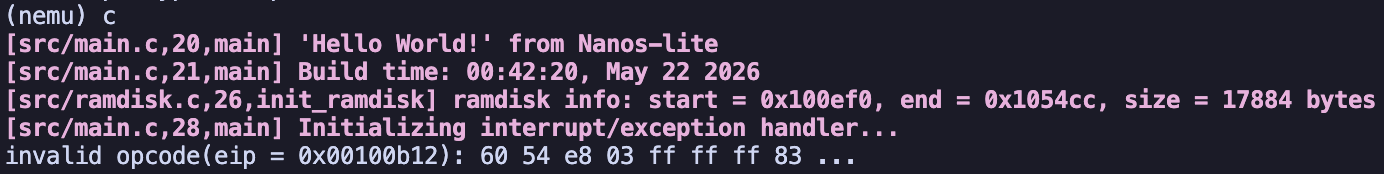
\includegraphics[width=0.82\textwidth]{pa3-vecsys-entry.png}
  \caption{中断机制已经把控制流推进到 \texttt{vecsys()} 异常入口附近}
  \label{fig:pa3-vecsys-entry}
\end{figure}

结合 \texttt{trap.S}：
\begin{lstlisting}[language={[x86masm]Assembler}]
vecsys:  pushl $0
         pushl $0x80
         jmp asm_trap

asm_trap:
         pushal
         pushl %esp
         call irq_handle
\end{lstlisting}
可以看出，当前系统已经成功完成了：
\[
\texttt{int \$0x80} \rightarrow \texttt{raise\_intr()} \rightarrow \texttt{vecsys()}
\]
新的阻塞点只是 \texttt{pushal/pusha} 还没有实现而已。因此，报告在这里可以明确给出阶段结论：看到未实现指令出现在 \texttt{vecsys()} 附近，并不是新的失败，而是说明 \texttt{lidt}、\texttt{int} 和 \texttt{raise\_intr()} 这一组中断机制已经实现正确，控制流已经成功进入系统调用异常入口。

\subsection{trap frame、\texttt{\_RegSet} 与系统调用参数传递}
这一部分先补的是 \texttt{pusha} 和 \texttt{popa}，因为 \texttt{vecsys()} 后面马上就会用到它们来构造和恢复通用寄存器现场。只有先把这两条指令的真实压栈/弹栈顺序做对，后面的 trap frame 才有稳定布局可言。

\texttt{pusha} 和 \texttt{popa} 在这里不能只写成“把寄存器全压下去/全弹回来”这么简单，因为它们本身就决定了后面 trap frame 的真实布局。当前工程里的实现是：
\begin{lstlisting}[language=C]
make_EHelper(pusha) {
  rtlreg_t old_esp = cpu.esp;
  rtl_push(&cpu.eax);
  rtl_push(&cpu.ecx);
  rtl_push(&cpu.edx);
  rtl_push(&cpu.ebx);
  rtl_push(&old_esp);
  rtl_push(&cpu.ebp);
  rtl_push(&cpu.esi);
  rtl_push(&cpu.edi);
}

make_EHelper(popa) {
  rtl_pop(&cpu.edi);
  rtl_pop(&cpu.esi);
  rtl_pop(&cpu.ebp);
  rtl_pop(&t0);
  rtl_pop(&cpu.ebx);
  rtl_pop(&cpu.edx);
  rtl_pop(&cpu.ecx);
  rtl_pop(&cpu.eax);
}
\end{lstlisting}

\texttt{pusha} 里最容易写错的是 \texttt{esp}。i386 手册要求压到第五个槽位上的必须是执行 \texttt{pusha} 之前的旧 \texttt{esp}，因此这里专门先用 \texttt{old\_esp} 把它存下来，再按 \texttt{eax, ecx, edx, ebx, old\_esp, ebp, esi, edi} 的顺序压栈。反过来，\texttt{popa} 恢复时虽然也会遇到那个 \texttt{esp} 槽位，但不能真的把它写回当前 \texttt{esp}，这里只是用 \texttt{rtl\_pop(\&t0)} 把这 4 个字节跳过去。也正因为这套顺序是固定的，后面的 \texttt{\_RegSet} 成员顺序也必须严格跟着它来。

这里正对应指导书里“实现 \texttt{pusha} 指令，并重新组织 \texttt{\_RegSet} 成员顺序，使它和 \texttt{trap.S} 构造出来的 trap frame 完全一致”这一要求。最开始把 \texttt{pusha} 接通之后，系统虽然已经能够一路推进到 \texttt{do\_event()}，但因为 \texttt{\_RegSet} 和真实压栈布局没有对齐，\texttt{do\_event()} 里读到的事件号是错误的，并且直接出现了：
\begin{center}
\texttt{Unhandled event ID = 8}
\end{center}
这正是讲义中提到的那个 \texttt{BAD TRAP} 检查点。它说明问题已经不再出在中断入口能不能跳到，而是出在 trap frame 被 C 代码解释时发生了错位。

这一阶段真正关键的工作，就是重新组织 \texttt{nexus-am/am/arch/x86-nemu/include/arch.h} 中的 \texttt{\_RegSet}，让它与 \texttt{trap.S} 中的压栈布局一一对应。只有这样，后续的事件号读取、\texttt{SYSCALL\_ARGx()} 宏取参数、系统调用返回值回写以及 \texttt{iret} 恢复现场才能全部对齐。

把 \texttt{\_RegSet} 重排到和汇编压栈顺序一致之后，异常现场才真正能够稳定推进到 \texttt{do\_event()}，如图 \ref{fig:pa3-do-event} 所示。

\begin{figure}[H]
  \centering
  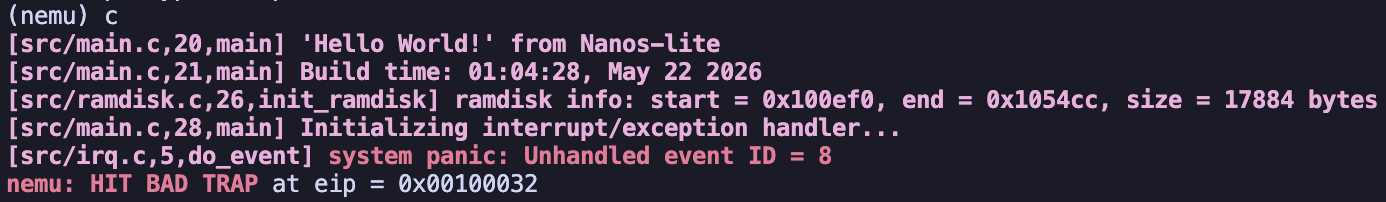
\includegraphics[width=0.82\textwidth]{pa3-do-event.png}
  \caption{异常入口、trap frame 构造和事件传递已经正确推进到 \texttt{do\_event()}}
  \label{fig:pa3-do-event}
\end{figure}

\subsection{实现 \texttt{SYS\_none}、\texttt{SYS\_exit} 与最小系统调用闭环}
这一部分先做的事情，是把 \texttt{\_EVENT\_SYSCALL} 在 \texttt{do\_event()} 里单独识别出来，并且把它送到 \texttt{do\_syscall()}。在这条分支真正接通之后，再继续补 \texttt{SYSCALL\_ARG1/2/3} 宏、返回固定值的 \texttt{SYS\_none}、系统调用返回值回写，以及最后会调用 \texttt{\_halt()} 的 \texttt{SYS\_exit}。这样一来，最小系统调用链路才算真正闭合。

\texttt{\_EVENT\_SYSCALL} 在当前代码里就是这样接进 \texttt{do\_event()} 的：
\begin{lstlisting}[language=C]
static _RegSet* do_event(_Event e, _RegSet* r) {
  switch (e.event) {
    case _EVENT_SYSCALL:
      return do_syscall(r);
    default:
      panic("Unhandled event ID = %d", e.event);
  }
}
\end{lstlisting}

这段代码表面很短，但它正好标出了“异常事件被识别成系统调用”这一时刻。前面如果 trap frame 顺序没对齐，或者 \texttt{irq\_handle()} 没把异常号正确包装成事件，这里看到的就不会是 \texttt{\_EVENT\_SYSCALL}，而会直接落进 \texttt{Unhandled event ID = 8} 这样的 \texttt{BAD TRAP}。因此，先把这条分支走通，本身就说明从 \texttt{trap.S} 到 \texttt{irq\_handle()} 再到 \texttt{do\_event()} 的事件传递链已经基本正确。

这一段在实现顺序上其实对应了指导书给出的整条返回路径：先让 \texttt{do\_event()} 正确识别 \texttt{\_EVENT\_SYSCALL}，再让 \texttt{SYSCALL\_ARGx()} 宏能够从 trap frame 里取到正确参数；随后补上 \texttt{SYS\_none}，验证“系统调用能够进入内核再返回用户态”；接着再实现 \texttt{popa} 和 \texttt{iret}，让恢复现场这一步真正成立；最后在 \texttt{dummy} 继续向前执行并触发 \texttt{SYS\_exit} 时，再补上 \texttt{SYS\_exit -> \_halt()}，于是程序就能最终走到 \texttt{GOOD TRAP}。

这里真正重要的是参数从哪里取、返回值写回哪里。在本次实现中，系统调用参数宏被写成了直接从 trap frame 对应寄存器字段里取值，例如：
\begin{lstlisting}[language=C]
#define SYSCALL_ARG1(r) ((r)->eax)
#define SYSCALL_ARG2(r) ((r)->ebx)
#define SYSCALL_ARG3(r) ((r)->ecx)
\end{lstlisting}

\texttt{do\_syscall()} 再根据这些宏完成最小分发：
\begin{lstlisting}[language=C]
static void do_syscall(_RegSet *r) {
  uintptr_t a[4];
  a[0] = SYSCALL_ARG1(r);
  a[1] = SYSCALL_ARG2(r);
  a[2] = SYSCALL_ARG3(r);

  switch (a[0]) {
    case SYS_none: r->eax = 1; break;
    case SYS_exit: _halt(a[1]); break;
  }
}
\end{lstlisting}

这里真正需要对齐的是 trap frame 和系统调用参数的对应关系。\texttt{a[0]}、\texttt{a[1]}、\texttt{a[2]} 分别从 trap frame 中取出系统调用号和参数，相当于重新解释用户态发起 \texttt{\_syscall\_()} 时放进寄存器里的值；进入 \texttt{switch} 之后，\texttt{SYS\_none} 把返回值写回 \texttt{r->eax}，于是用户程序回到用户态后就能从 \texttt{eax} 读到结果；而 \texttt{SYS\_exit} 直接调用 \texttt{\_halt()}，则表示这个系统调用不会再返回到原用户程序。

这样实现的原因是，用户态和内核态之间没有共享函数调用栈，内核不能直接继续用户函数的执行。正确做法只能是：先从 trap frame 中把参数提取出来，在内核里完成服务，再把结果重新写回 trap frame 中约定的寄存器位置，最后由 \texttt{iret} 恢复回用户态。也正因为如此，trap frame 的字段顺序、系统调用参数宏和返回值写回位置必须全部对应起来。

重新运行 \texttt{dummy} 后，系统终于可以不再停在异常机制内部，而是完整地完成一次系统调用并返回，然后进一步执行到 \texttt{GOOD TRAP}。对应截图如图 \ref{fig:pa3-syscall-good-trap} 所示。

\begin{figure}[H]
  \centering
  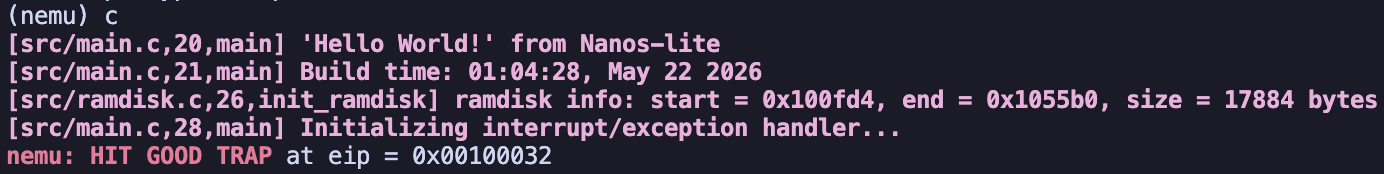
\includegraphics[width=0.82\textwidth]{pa3-syscall-good-trap.png}
  \caption{最小系统调用闭环完成后，\texttt{dummy} 顺利执行到 \texttt{GOOD TRAP}}
  \label{fig:pa3-syscall-good-trap}
\end{figure}

到这一步为止，PA3 的第二阶段已经建立起一条完整链路：
\[
\texttt{\_start()} \rightarrow \texttt{int \$0x80} \rightarrow \texttt{trap frame} \rightarrow \texttt{do\_syscall()} \rightarrow \texttt{iret}
\]
这条链是后续所有文件系统和设备访问能力的前提。若按指导书中的阶段划分来看，\texttt{dummy} 在这里输出 \texttt{GOOD TRAP}，就意味着 PA3 的阶段 1 已经完成。本报告前面把 raw loader、中断机制和系统调用闭环拆开写，主要是为了把每个阻塞点和对应修改解释得更清楚。

\section{文件系统、设备抽象与运行完整用户程序}

\subsection{实现 \texttt{SYS\_write} 与在 Nanos-lite 上运行 \texttt{hello}}
有了最小系统调用闭环之后，下一步最自然的目标就是让用户程序输出。因为无论是 \texttt{puts()} 还是 \texttt{printf()}，最终都要依赖 \texttt{write()} 系统调用。

在 \texttt{nanos-lite/src/syscall.c} 中补上 \texttt{SYS\_write} 之后，再将 \texttt{hello} 打包进 \texttt{ramdisk} 并运行，最终可以看到用户层字符串已经通过系统调用链路输出到了串口。对应截图如图 \ref{fig:pa3-hello-output} 所示。

这一部分的核心代码骨架其实很直接：
\begin{lstlisting}[language=C]
case SYS_write:
  if (a[1] == 1 || a[1] == 2) {
    _putc((char *)a[2], a[3]);
    r->eax = a[3];
  }
  break;
\end{lstlisting}

如果按系统调用语义来理解，\texttt{a[1]} 对应文件描述符，\texttt{a[2]} 对应用户缓冲区地址，\texttt{a[3]} 对应本次要写出的字节数。这里先判断文件描述符是否为 \texttt{stdout} 或 \texttt{stderr}，因为 \texttt{hello} 阶段最先需要支持的只是把字符串输出到终端；条件成立后，就把用户缓冲区中的内容交给底层串口输出函数，再把实际写出的字节数写回 \texttt{r->eax}，作为用户态看到的返回值。

这里先把 \texttt{stdout/stderr} 接通，优先验证 \texttt{hello} 的输出路径。这样一来，只要 \texttt{SYS\_write} 能让 \texttt{hello} 正常打印，就可以确认从 \texttt{libos} 发起 \texttt{write()}、经由 \texttt{int \$0x80} 陷入、再到内核解释参数并返回结果这一整条链路已经闭合。后面的普通文件写入，再沿着同一套分发框架继续扩展即可。

\begin{figure}[H]
  \centering
  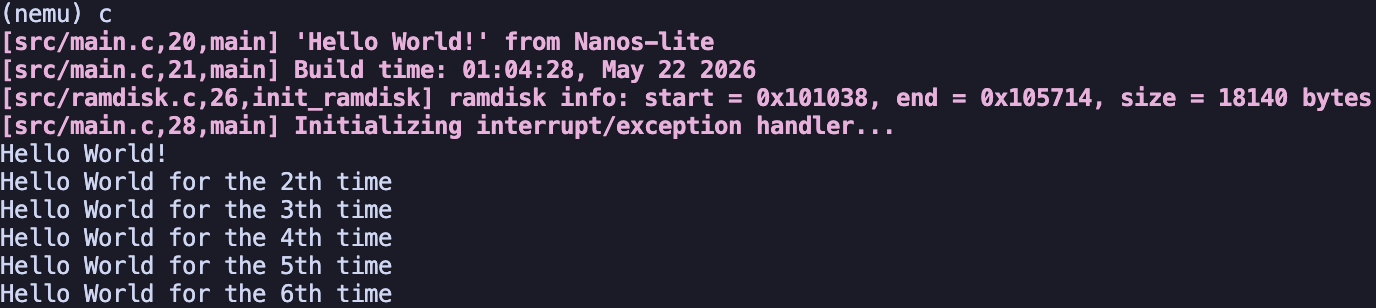
\includegraphics[width=0.82\textwidth]{pa3-hello-output.png}
  \caption{\texttt{SYS\_write} 实现后，\texttt{hello} 已经能在 Nanos-lite 上正常输出}
  \label{fig:pa3-hello-output}
\end{figure}

走到这里之后，操作系统已经不再只是负责把用户程序装进内存，用户程序开始通过系统调用真正使用内核提供的服务。

\subsection{实现 \texttt{SYS\_brk} 与用户层 \texttt{\_sbrk()}}
仅仅输出还不够，因为后面的 \texttt{printf()}、\texttt{malloc()}、文件 I/O 缓冲都可能依赖堆区增长。因此还需要在内核和用户层同时接通 \texttt{brk/sbrk}：用户层的 \texttt{\_sbrk()} 先根据 \texttt{increment} 计算新的 program break，再通过 \texttt{SYS\_brk} 请求内核修改 break，而当前 PA3 阶段可以先把 \texttt{SYS\_brk} 简化成总是返回成功。

\texttt{brk} 这一部分还谈不上完整内存管理，但已经足够让 \texttt{libc/libos} 的堆区相关代码继续工作，后面的标准库输出和文件操作也因此有了基础。

\subsection{实现简易文件系统并运行 \texttt{text}}
文件系统这一段是分几步补起来的。先确认 \texttt{files.h} 生成的静态文件表里已经记录了文件名、大小和 \texttt{ramdisk} 偏移；然后在 \texttt{fs\_open()} 中加入按文件名线性查找并返回文件描述符；接着在 \texttt{fs\_read()} 中按 \texttt{open\_offset} 调用 \texttt{ramdisk\_read()}，在 \texttt{fs\_write()} 中先处理 \texttt{stdout/stderr} 再处理普通文件；最后再把 \texttt{fs\_lseek()} 和 \texttt{fs\_filesz()} 接齐，并让 \texttt{loader()} 改成通过 \texttt{fs\_open()/fs\_read()} 按文件名装载程序。

在这些操作中，\texttt{fs\_open()} 负责按路径在静态文件表中查找文件，\texttt{fs\_read()} 与 \texttt{fs\_write()} 负责基于 \texttt{ramdisk\_read()} / \texttt{ramdisk\_write()} 访问普通文件，\texttt{fs\_lseek()} 维护文件当前偏移，而 \texttt{fs\_close()} 与 \texttt{fs\_filesz()} 则把剩余的关闭与长度查询接口补齐。

其中最核心的一段代码其实是 \texttt{fs\_read()}，因为它把文件描述符和当前偏移真正翻译成了对 \texttt{ramdisk} 的读取：
\begin{lstlisting}[language=C]
size_t fs_read(int fd, void *buf, size_t len) {
  size_t left = file_table[fd].size - file_table[fd].open_offset;
  if (len > left) len = left;
  ramdisk_read(buf,
    file_table[fd].disk_offset + file_table[fd].open_offset, len);
  file_table[fd].open_offset += len;
  return len;
}
\end{lstlisting}

如果按执行顺序看，这段代码先通过 \texttt{size - open\_offset} 计算文件剩余可读内容，避免越过文件末尾；接着如果请求的 \texttt{len} 比剩余字节还大，就把本次读取长度截断到合法范围；随后用 \texttt{disk\_offset + open\_offset} 算出这次在 \texttt{ramdisk} 中真正应该读取的位置，再把数据搬到用户提供的缓冲区；最后将 \texttt{open\_offset} 增加本次读取的长度，为下次连续读取做好准备。

\texttt{open\_offset} 在这里必须管起来。只有把当前偏移和文件描述符绑定，\texttt{read()} 才能表现成一个有状态的顺序读取接口。后面的普通文件访问、\texttt{pal} 资源加载以及通过文件名装载用户程序，才能共用同一套基础设施。

为了让这里的实现过程更直观，报告中再补一段当前代码里的 \texttt{fs\_open()} 与 \texttt{fs\_read()}。这两段代码正好把文件名查找、偏移初始化和顺序读取的逻辑连在了一起：
\begin{lstlisting}[language=C]
int fs_open(const char *pathname, int flags, int mode) {
  for (int i = 0; i < NR_FILES; i++) {
    if (strcmp(file_table[i].name, pathname) == 0) {
      file_table[i].open_offset = 0;
      return i;
    }
  }
  assert(0);
  return -1;
}

size_t fs_read(int fd, void *buf, size_t len) {
  if (file_table[fd].open_offset + len > file_table[fd].size) {
    len = file_table[fd].size - file_table[fd].open_offset;
  }
  ramdisk_read(buf,
      file_table[fd].disk_offset + file_table[fd].open_offset, len);
  file_table[fd].open_offset += len;
  return len;
}
\end{lstlisting}

\texttt{fs\_open()} 做的事情并不复杂，就是在静态文件表里按名字查找目标文件，并在找到之后把 \texttt{open\_offset} 清零。这个动作很重要，因为像 \texttt{/proc/dispinfo} 这样的特殊文件会被反复打开，偏移不重置的话第二次打开就可能直接落到 EOF。下面的 \texttt{fs\_read()} 则把顺序读取真正落实下来：先根据文件大小截断本次读取长度，再用 \texttt{disk\_offset + open\_offset} 算出当前应该从 \texttt{ramdisk} 的哪个位置取数据，最后把 \texttt{open\_offset} 向前推进。这里的代码虽然短，但已经把文件描述符和当前位置一起工作的读取方式表达得很完整。

实现文件系统之后，\texttt{loader()} 也从固定读取 \texttt{ramdisk} 偏移 \texttt{0} 升级成通过文件名读取指定程序文件。这一步非常重要，因为从此之后，\texttt{/bin/hello}、\texttt{/bin/text}、\texttt{/bin/pal} 等程序都可以通过同一套接口装载，而不再依赖硬编码偏移。

使用 \texttt{/bin/text} 验证文件系统后，程序顺利输出 \texttt{PASS!!!}，对应截图如图 \ref{fig:pa3-text-pass} 所示。

\begin{figure}[H]
  \centering
  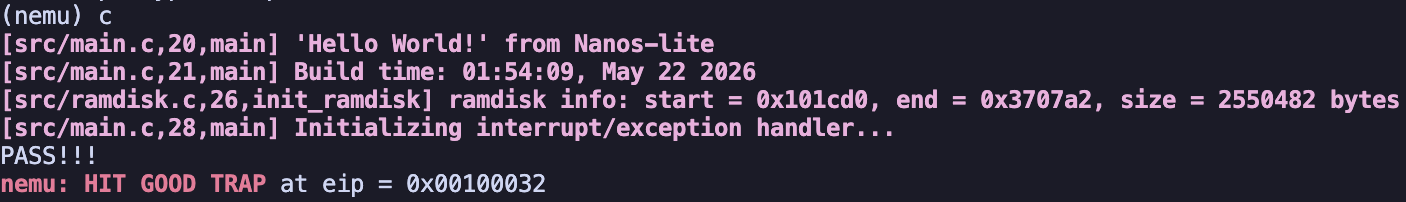
\includegraphics[width=0.82\textwidth]{pa3-text-pass.png}
  \caption{简易文件系统与 \texttt{text} 验证通过}
  \label{fig:pa3-text-pass}
\end{figure}

按指导书中的阶段划分，做到这里时，PA3 阶段 2 实际上已经完成。原因很直接：\texttt{loader} 已经从直接调用 \texttt{ramdisk\_read()} 改成了通过 \texttt{fs\_open()/fs\_read()/fs\_close()} 按文件名装载程序；\texttt{fs\_write()} 和 \texttt{fs\_lseek()} 也已经补齐；而 \texttt{/bin/text} 输出 \texttt{PASS!!!} 则说明这套文件读写与定位接口已经可以正确工作。本报告后面继续往下写设备文件和 \texttt{pal}，属于把指导书后续内容顺着实现链路展开，而不是仍然停留在阶段 2 内部。

\subsection{将设备抽象为文件}
PA3 后半段最有操作系统味道的一部分，是把设备也抽象为文件接口。根据指导书，这里实现了三类关键设备文件：\texttt{/dev/fb} 用来映射屏幕 frame buffer，供用户程序写像素；\texttt{/proc/dispinfo} 用来向用户程序暴露屏幕宽高信息；\texttt{/dev/events} 则向用户程序提供按键事件和时间事件。

其中，\texttt{/dev/fb} 的核心是根据写入偏移换算屏幕坐标，再调用 AM 的 \texttt{\_draw\_rect()}；\texttt{/proc/dispinfo} 本质上就是一段由内核拼好的只读字符串；\texttt{/dev/events} 则会优先返回按键事件，没有按键时再返回时钟事件。这样做之后，普通文件和设备文件在用户态都统一落到：
\[
\texttt{open/read/write/lseek/close}
\]
这套接口上。

为了让这部分实现过程更具体，这里可以把 \texttt{/dev/fb} 和 \texttt{/dev/events} 的核心逻辑分别看成把用户层字节流请求翻译成设备动作，以及把设备状态重新包装成可读字符串两件事。一个典型的 \texttt{fb\_write()} 骨架如下：
\begin{lstlisting}[language=C]
size_t fb_write(const void *buf, size_t offset, size_t len) {
  int x = (offset / 4) % screen_w;
  int y = (offset / 4) / screen_w;
  int w = len / 4;
  _draw_rect((uint32_t *)buf, x, y, w, 1);
  return len;
}
\end{lstlisting}

这段代码里，\texttt{offset} 的单位本来是相对 frame buffer 开头的字节偏移，而屏幕绘制接口需要的却是坐标和像素块。因此前两行先把字节偏移换算成像素编号，再进一步换算成二维坐标 \texttt{(x, y)}；\texttt{len / 4} 表示本次写入包含多少个 32 位像素；最后把用户缓冲区中的像素数据直接交给 \texttt{\_draw\_rect()} 绘制到屏幕上。\texttt{/dev/fb} 对用户仍然表现成文件写入，内核内部则把这次写操作翻译成一次图形输出动作。

而 \texttt{/dev/events} 的实现重点则在于把当前是否存在按键事件转成用户程序可读的一行文本，一个典型骨架如下：
\begin{lstlisting}[language=C]
size_t events_read(void *buf, size_t offset, size_t len) {
  _Event e = _read_key();
  if (e.event == _KEY_NONE) return 0;
  return snprintf(buf, len, "kd %s\n", keyname[e.keycode]);
}
\end{lstlisting}

这里的第一步不是直接返回某个硬件寄存器值，而是先通过 AM 读取一次抽象后的按键事件；如果当前没有按键，就返回 \texttt{0}，表示这次读取没有得到内容；一旦有键盘事件，就把它重新格式化成用户程序约定的字符串形式。用户态程序并不需要理解底层扫描码，而是像读普通文本文件一样，按行取得按键按下或释放信息。设备文件抽象的价值也正好体现在这里：底层是硬件事件，用户看到的是统一的 \texttt{read()} 接口。

使用 \texttt{bmptest} 验证图形输出后，系统能够正确显示 Project-N Logo，如图 \ref{fig:pa3-bmptest-logo} 所示。

\begin{figure}[H]
  \centering
  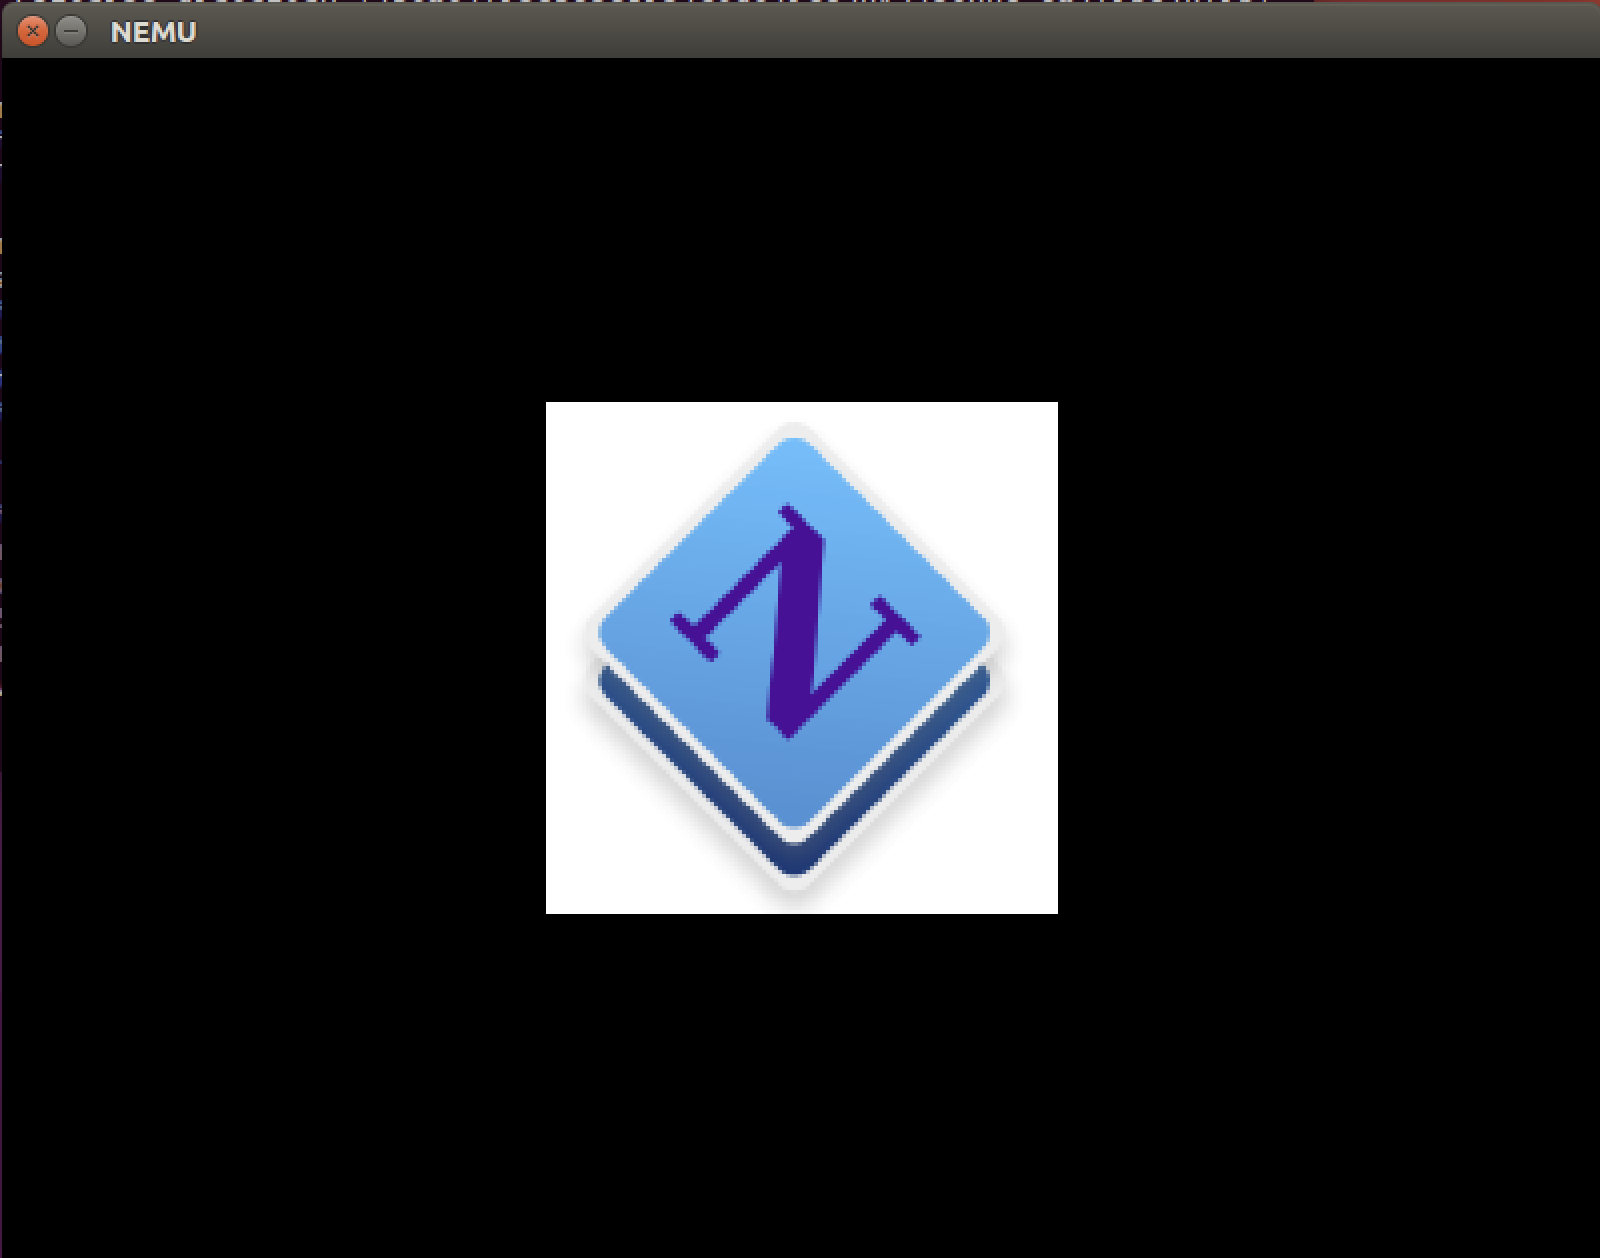
\includegraphics[width=0.68\textwidth]{pa3-bmptest-logo.png}
  \caption{\texttt{bmptest} 成功通过 \texttt{/dev/fb} 与 \texttt{/proc/dispinfo} 显示 Project-N Logo}
  \label{fig:pa3-bmptest-logo}
\end{figure}

使用 \texttt{events} 或相关调试输出验证输入事件后，也可以看到键盘事件已经能够通过 \texttt{/dev/events} 正确上送，如图 \ref{fig:pa3-events-debug} 所示。

\begin{figure}[H]
  \centering
  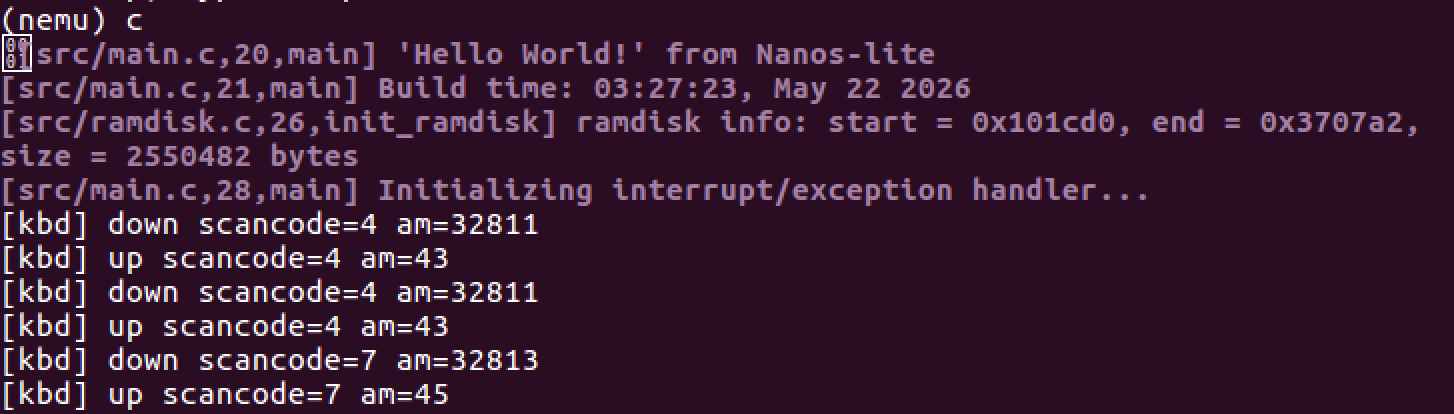
\includegraphics[width=0.82\textwidth]{pa3-events-debug.png}
  \caption{键盘事件已经能够经由 \texttt{/dev/events} 返回给用户程序}
  \label{fig:pa3-events-debug}
\end{figure}

\subsection{运行 \texttt{pal}}
当文件系统和设备文件全部贯通之后，PA3 的最终用户程序目标就是 \texttt{pal}。这一步对系统的要求已经明显高于 \texttt{dummy}、\texttt{hello} 和 \texttt{text}，因为 \texttt{pal} 同时依赖程序本体装载、资源文件读取、帧缓冲输出、屏幕信息接口、键盘事件接口以及标准库和堆区支持。也就是说，前面分别做通的几条主线，到这里第一次真正汇合到同一个用户程序上。

\texttt{pal} 能跑起来，最前面的入口仍然是 \texttt{loader()}。这里在 \texttt{nanos-lite/src/loader.c} 中把原来“从固定 \texttt{ramdisk} 偏移直接搬整段程序”的写法改成了“先按文件名打开，再按文件大小读取”的版本。这样一来，\texttt{/bin/pal}、\texttt{/bin/text}、\texttt{/bin/hello} 都可以沿着同一套接口装载。对应逻辑可以写成：
\begin{lstlisting}[language=C]
uintptr_t loader(_Protect *as, const char *filename) {
  int fd = fs_open(filename, 0, 0);
  size_t size = fs_filesz(fd);
  fs_read(fd, DEFAULT_ENTRY, size);
  fs_close(fd);
  return (uintptr_t)DEFAULT_ENTRY;
}
\end{lstlisting}

这一段虽然不长，但它把 \texttt{/bin/pal} 的装载过程彻底从硬编码偏移改成了按文件名查找并读取。\texttt{fs\_open(filename, 0, 0)} 先在静态文件表里找到 \texttt{/bin/pal}，\texttt{fs\_filesz(fd)} 拿到程序长度，随后 \texttt{fs\_read(fd, DEFAULT\_ENTRY, size)} 把整个程序搬到用户入口地址。前面已经补好的 \texttt{fs\_open()}、\texttt{fs\_read()} 和 \texttt{open\_offset} 管理，到了这里不再只是文件系统功能本身，而是直接参与了用户程序装载。

\texttt{pal} 进入执行之后，最先依赖的不是单一一个接口，而是一整组设备文件初始化是否到位。这里在 \texttt{nanos-lite/src/fs.c} 中写了 \texttt{init\_fs()}，在 \texttt{nanos-lite/src/device.c} 中写了 \texttt{init\_device()}，两者分别负责把 frame buffer 大小和屏幕信息准备好：
\begin{lstlisting}[language=C]
void init_fs() {
  file_table[FD_FB].size = _screen.height * _screen.width * 4;
}

void init_device() {
  _ioe_init();
  sprintf(dispinfo, "WIDTH:%d\nHEIGHT:%d\n",
      _screen.width, _screen.height);
}
\end{lstlisting}

\texttt{init\_fs()} 里这句 \texttt{file\_table[FD\_FB].size = height * width * 4}，是这里手动补进去的关键一行。它把 \texttt{/dev/fb} 的大小设置成整块屏幕像素数组的字节数，这样用户程序后面才能把 frame buffer 当成一个普通可写文件来使用。下面的 \texttt{init\_device()} 则在设备层初始化完成后，用 \texttt{sprintf()} 把屏幕宽高拼成一段字符串放进 \texttt{dispinfo}，于是 \texttt{/proc/dispinfo} 后续只需要按偏移读出这段字符串即可。对 \texttt{pal} 来说，这两部分分别对应图形输出和窗口尺寸信息，缺少任何一项，初始化都走不下去。

除了程序本体，\texttt{pal} 运行时还会持续读取大量资源文件，这一部分依赖的仍然是前面已经搭好的文件系统路径。这里在 \texttt{nanos-lite/src/fs.c} 中真正补出来的关键函数是 \texttt{fs\_read()}，当前它在普通文件上的处理逻辑如下：
\begin{lstlisting}[language=C]
default:
  ramdisk_read(buf,
    file_table[fd].disk_offset + file_table[fd].open_offset, len);
  file_table[fd].open_offset += len;
  break;
\end{lstlisting}

这几行代码正好对应了 \texttt{pal} 资源加载时最核心的动作。这里写进去的第一句 \texttt{ramdisk\_read(...)} 把普通文件读取真正落到了 \texttt{ramdisk} 上，第二句 \texttt{file\_table[fd].open\_offset += len} 则把文件当前偏移向前推进。打开某个资源文件之后，\texttt{fd} 已经确定了它在文件表中的位置，\texttt{disk\_offset} 给出这个文件在 \texttt{ramdisk} 中的起始偏移，\texttt{open\_offset} 表示当前已经读到了文件里的哪个位置。于是每次读取时，只需要把两者相加，就能在 \texttt{ramdisk} 中找到真正应该读取的数据位置。资源文件很多，但这套逻辑不需要为每一种资源单独写读取函数，\texttt{pal} 的图片、脚本和数据文件都沿着同一条路径进入内存。

\texttt{pal} 的图形显示部分，则直接落到 \texttt{/dev/fb} 和 \texttt{/proc/dispinfo} 这两个设备文件上。这里在 \texttt{nanos-lite/src/device.c} 中补上的 \texttt{fb\_write()}，真正把用户层的写文件请求翻译成了屏幕绘制：
\begin{lstlisting}[language=C]
void fb_write(const void *buf, off_t offset, size_t len) {
  int row = (offset / 4) / _screen.width;
  int col = (offset / 4) % _screen.width;
  _draw_rect(buf, col, row, len / 4, 1);
}
\end{lstlisting}

\texttt{pal} 写 frame buffer 时，用户态看到的是往某个文件偏移写一段数据，到了内核里，这里写进去的 \texttt{row} 和 \texttt{col} 计算会先把字节偏移换算成屏幕上的行列坐标，最后再调用 \texttt{\_draw\_rect()} 把像素真正画到窗口上。也就是说，\texttt{pal} 并没有直接操作某个显存寄存器，而是通过文件写接口完成图形输出。前面说设备也可以抽象成文件，到这里就已经不是概念解释，而是直接体现在游戏画面刷新上。

输入这条线同样不能缺。这里在 \texttt{nanos-lite/src/device.c} 中补出来的 \texttt{events\_read()}，会把底层键盘事件重新包装成用户程序能够按行读取的文本：
\begin{lstlisting}[language=C]
if (key == _KEY_NONE) {
  unsigned long t = _uptime();
  sprintf(buf, "t %d\n", t);
} else {
  sprintf(buf, "%s %s\n", down ? "kd" : "ku", keyname[key]);
}
\end{lstlisting}

如果当前没有按键，这里就用 \texttt{\_uptime()} 和 \texttt{sprintf()} 生成一条时间事件；一旦有按键，就返回形如 \texttt{kd KEYNAME} 或 \texttt{ku KEYNAME} 的字符串。对 \texttt{pal} 来说，这意味着输入系统不必自己理解底层扫描码，而是像读取普通文本一样，直接得到某个键被按下或释放的事件描述。这样做虽然很朴素，但已经足够支撑游戏运行时的键盘输入逻辑。

从实现顺序上看，\texttt{pal} 能够跑起来，大致经历了这样一条组合链：这里先在 \texttt{loader.c} 中把 \texttt{/bin/pal} 程序本体装入内存；随后在 \texttt{fs.c} 中通过 \texttt{fs\_open()/fs\_read()} 反复读取资源文件；图形输出在 \texttt{device.c} 中通过 \texttt{/dev/fb} 落到 \texttt{fb\_write()}；屏幕尺寸信息通过 \texttt{/proc/dispinfo} 提供；输入事件则通过 \texttt{/dev/events} 返回给用户程序；标准库和堆区逻辑则由前面已经接通的 \texttt{SYS\_write} 和 \texttt{SYS\_brk} 兜底。只有这些部分一起工作时，\texttt{pal} 才会从能装入内存，真正走到能显示、能读资源、能处理输入的状态。

最终远端运行结果表明 \texttt{pal} 已经能够成功初始化并进入运行状态，对应截图如图 \ref{fig:pa3-pal-success} 所示。

\begin{figure}[H]
  \centering
  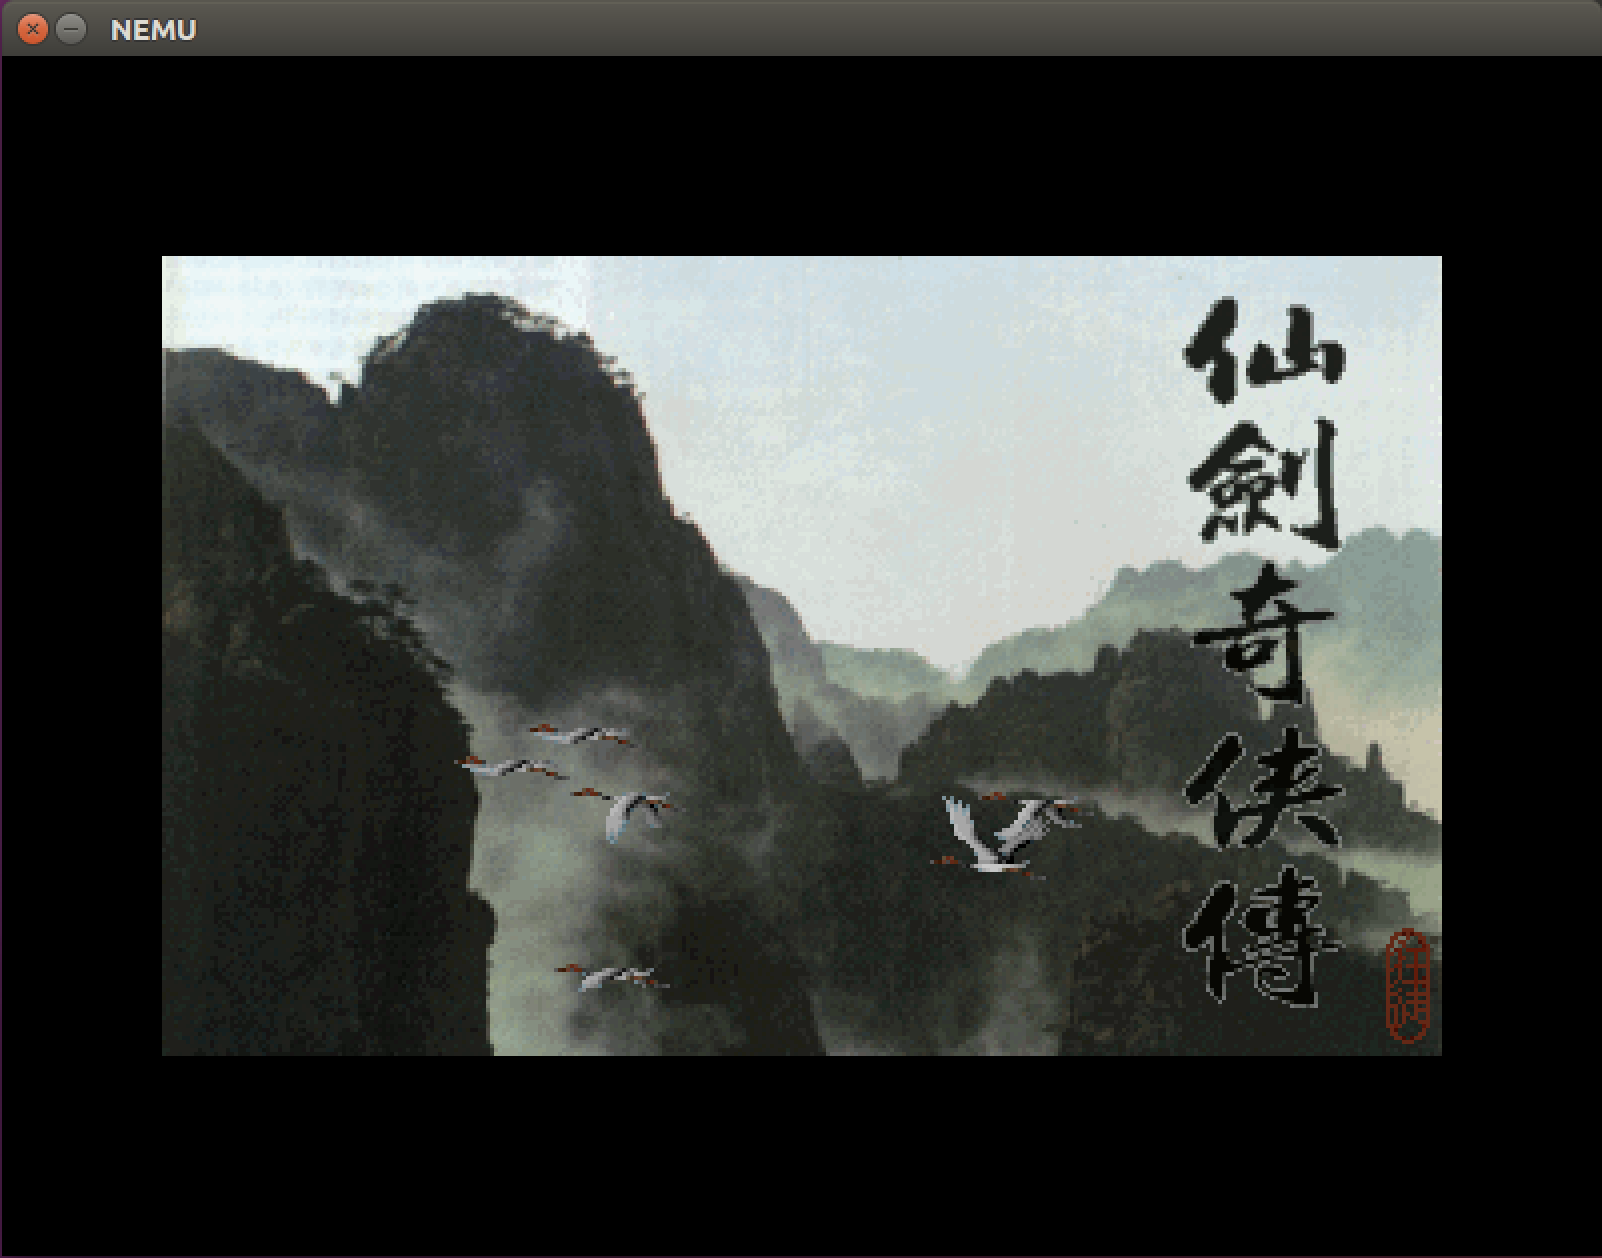
\includegraphics[width=0.72\textwidth]{pa3-pal-success.png}
  \caption{\texttt{pal} 成功运行，说明 PA3 的文件系统与设备抽象主线已经打通}
  \label{fig:pa3-pal-success}
\end{figure}

\section{必答题}

\subsection{仙剑奇侠传中游戏存档的读取过程}
在 \texttt{navy-apps/apps/pal/src/global/global.c} 的 \texttt{PAL\_LoadGame()} 中，游戏存档的读取代码很直接：
\begin{lstlisting}[language=C]
fp = fopen(szFileName, "rb");
fread(&s, sizeof(SAVEDGAME), 1, fp);
fclose(fp);
\end{lstlisting}

表面上看，这里只是三行标准 C 文件操作；真正的调用链却横跨了仙剑程序、库函数、libos、Nanos-lite、AM 和 NEMU 六层。最上层的仙剑程序先调用 \texttt{fopen()} 打开存档文件，再调用 \texttt{fread()} 读取一个 \texttt{SAVEDGAME} 结构，最后 \texttt{fclose()} 关闭文件。这里的 \texttt{fread()} 来自 libc，它本身不会直接访问磁盘，而是通过底层文件对象反复向更低层请求数据。newlib 的 \texttt{fread()} 最终依赖的是操作系统提供的 \texttt{read}、\texttt{lseek} 这类基本接口。

libos 这一层正好把这些标准库调用转换成系统调用。当前工程里的 \texttt{libos/src/nanos.c} 中，\texttt{\_read()} 的实现就是：
\begin{lstlisting}[language=C]
int _read(int fd, void *buf, size_t count) {
  return _syscall_(SYS_read, fd, (uintptr_t)buf, count);
}
\end{lstlisting}

也就是说，libc 里的 \texttt{fread()} 最终会落到 \texttt{\_read()}，再通过 \texttt{int \$0x80} 发起 \texttt{SYS\_read} 系统调用。进入 Nanos-lite 之后，\texttt{do\_syscall()} 会根据系统调用号把请求分发给文件系统：
\begin{lstlisting}[language=C]
case SYS_read:
  r->eax = fs_read(a[1], (void *)a[2], a[3]);
  break;
\end{lstlisting}

真正完成存档读取的是 \texttt{fs\_read()}。对于普通文件，它会根据文件描述符在静态文件表中找到该文件的 \texttt{disk\_offset} 和当前 \texttt{open\_offset}，然后调用 \texttt{ramdisk\_read()}：
\begin{lstlisting}[language=C]
ramdisk_read(buf,
  file_table[fd].disk_offset + file_table[fd].open_offset, len);
file_table[fd].open_offset += len;
\end{lstlisting}

这两行代码把“读存档文件”真正翻译成了“从 ramdisk 的某个偏移把一段字节复制到用户缓冲区”。这里的 \texttt{disk\_offset} 表示这个存档文件在 ramdisk 中的起始位置，\texttt{open\_offset} 表示当前已经读到了文件里的哪个位置，因此两者相加之后，就能定位到本次读取在 ramdisk 中的真实地址。再往下看，\texttt{ramdisk\_read()} 实际就是把这一段数据从 NEMU 模拟内存中的 ramdisk 区域复制出来。也就是说，NEMU 在这一条链上承担的是底层内存和设备模拟者的角色，真正的数据最终还是从它维护的那片内存区域中被取出来。

如果把这一整条链路顺着写下来，就是：
\[
\texttt{PAL\_LoadGame() -> fread() -> \_read() -> SYS\_read ->}
\]

\[
\texttt{fs\_read() -> ramdisk\_read() -> NEMU\ memory}
\]

最上层程序提出“我要读这个文件”，标准库把它包装成文件流操作，libos 把它翻译成系统调用，Nanos-lite 再把它解释成对 ramdisk 文件的读取，最终由 NEMU 提供底层内存中的实际数据。

\subsection{仙剑奇侠传中屏幕更新的过程}
在 \texttt{navy-apps/apps/pal/src/hal/hal.c} 的 \texttt{redraw()} 中，游戏画面刷新同样写得非常直接：
\begin{lstlisting}[language=C]
NDL_DrawRect(fb, 0, 0, W, H);
NDL_Render();
\end{lstlisting}

这两行表明，仙剑程序本身并不直接操作显存或设备寄存器，而是把整张帧缓冲交给 NDL 去绘制。往下一层看，\texttt{NDL\_DrawRect()} 位于 \texttt{libs/libndl/src/ndl.c}，它先把应用传进来的像素写入 libndl 维护的 \texttt{canvas}，而真正把数据送给操作系统的是后面的 \texttt{NDL\_Render()}：
\begin{lstlisting}[language=C]
for (int i = 0; i < canvas_h; i ++) {
  fseek(fbdev, ((i + pad_y) * screen_w + pad_x) * sizeof(uint32_t), SEEK_SET);
  fwrite(&canvas[i * canvas_w], sizeof(uint32_t), canvas_w, fbdev);
}
\end{lstlisting}

这段代码说明 libndl 并不是一次性调用某个“画图系统调用”，而是把屏幕更新抽象成了对 \texttt{/dev/fb} 这个设备文件的多次 \texttt{fseek + fwrite}。也就是说，游戏画面最终被拆成了一行一行的像素写入。这里的 \texttt{fbdev} 就是通过 \texttt{fopen("/dev/fb", "w")} 打开的设备文件。

再往下一层看，libos 会把 \texttt{fwrite()} 触发的底层写操作转换成 \texttt{SYS\_write}。Nanos-lite 在 \texttt{do\_syscall()} 中把它分发给 \texttt{fs\_write()}，而 \texttt{fs\_write()} 对 \texttt{/dev/fb} 做了专门处理：
\begin{lstlisting}[language=C]
case FD_FB:
  fb_write(buf, file_table[fd].open_offset, len);
  file_table[fd].open_offset += len;
  break;
\end{lstlisting}

到了 \texttt{device.c} 里的 \texttt{fb\_write()}，这次“往文件某个偏移写一串字节”会被翻译成真正的屏幕坐标和像素块绘制：
\begin{lstlisting}[language=C]
void fb_write(const void *buf, off_t offset, size_t len) {
  int row = (offset / 4) / _screen.width;
  int col = (offset / 4) % _screen.width;
  _draw_rect(buf, col, row, len / 4, 1);
}
\end{lstlisting}

\texttt{offset / 4} 先把字节偏移换算成像素编号，再根据屏幕宽度拆成行号和列号；\texttt{len / 4} 表示本次写入包含多少个 32 位像素；最后调用 AM 提供的 \texttt{\_draw\_rect()} 把这一行像素真正交给底层设备接口。AM 在这里扮演的是硬件抽象层角色：上层不直接面对 NEMU 的设备寄存器，而是通过 \texttt{\_draw\_rect()} 这种统一接口完成显示更新。再往下，NEMU 负责模拟设备和显存，把这次绘制最终落实到模拟出来的显示设备状态上。

因此，屏幕更新这条链可以概括成：
\[
\texttt{redraw() -> NDL\_DrawRect() -> NDL\_Render() -> fwrite(/dev/fb)}
\]

\[
\rightarrow
\texttt{SYS\_write -> fs\_write() -> fb\_write() -> \_draw\_rect() -> NEMU\ device}
\]

这条链路说明仙剑奇侠传、库函数、libos、Nanos-lite、AM 和 NEMU 在画面更新时也是逐层协作的。最上层游戏只关心“把这块像素画出来”，libndl 把它整理成对 \texttt{/dev/fb} 的文件写入，libos 把写文件动作变成系统调用，Nanos-lite 识别出这是 frame buffer 设备文件，再由 AM 和 NEMU 把它落实成真正的设备更新。

\section{思考}
PA3 最值得记录的一个变化，是这里第一次明显感受到把程序跑起来和把系统做通并不是同一件事。单看某一个功能点，例如实现 \texttt{int}、补一个 \texttt{SYS\_write}，都像是在填局部空缺；但只要把这些局部点放回整条执行链，就会发现每一步都在依赖上一层的约定是否已经成立。也正因为如此，PA3 的调试过程并不适合靠猜，而更适合不断观察阻塞点向前推进：先从 \texttt{invalid opcode} 推到 \texttt{lidt}，再推进到 \texttt{vecsys()}、\texttt{do\_event()}，最后推进到 \texttt{GOOD TRAP} 和完整用户程序。

另一个比较重要的体会，是异常控制流并不只是硬件帮忙跳转一次这么简单。真正让系统调用成立的，是硬件现场保存、汇编压栈布局、C 语言结构体解释和内核分发逻辑之间的一整套配合。如果其中任意一层对同一块内存的理解不一致，例如 \texttt{\_RegSet} 成员顺序和 \texttt{trap.S} 压栈顺序不一致，那么最后表现出来的问题往往并不是直接崩溃，而是事件号错误、参数错位、返回值异常这类更难定位的现象。这个过程也使得 PA3 不再只是补指令，而是真正开始涉及系统接口约定的维护。

\subsection{对比异常与函数调用}
指导书里还专门提到一个值得对比的问题：函数调用和异常处理都会在控制流切换前保存现场，但两者保存的信息量并不一样。普通函数调用通常只需要保存返回地址，以及调用约定中要求由调用者保存的那部分寄存器。这是因为函数调用发生在程序自己可预期的执行逻辑中，调用方和被调用方对当前代码段、标志寄存器以及执行上下文有共同约定，很多状态默认不会在调用过程中被破坏。

异常处理则不同。异常或中断可能发生在一条普通指令执行之后，也可能来自用户程序主动发起的 \texttt{int \$0x80}，这时处理器必须把当前执行位置之外的更多上下文一起保留下来。除了返回地址，还要保存 \texttt{EFLAGS}、\texttt{CS}，后续 \texttt{trap.S} 还会继续保存通用寄存器，必要时还要连错误码、异常号一起纳入 trap frame。原因在于异常处理不是一次普通的子程序调用，而是处理器执行流被打断后切到另一段语义完全不同的代码路径；等这段处理代码结束时，系统还需要有能力把原来的执行环境原封不动地恢复回去。也正因为这一点，函数调用依赖的是调用约定，而异常处理依赖的是一整套由硬件压栈顺序、汇编入口和 trap frame 结构共同定义的现场保存约定。

\subsection{\texttt{trap.S} 里为什么要 \texttt{pushl \%esp}}
指导书里提到 \texttt{trap.S} 中那句 \texttt{pushl \%esp} 看起来很诡异，但结合前后代码之后，它的作用其实很直接。前面 \texttt{pushal} 和之前压入的错误码、异常号已经在当前内核栈上构造出了一整份 trap frame，这时的 \texttt{\%esp} 正好指向这份 trap frame 的起始位置。于是：
\begin{lstlisting}[language={[x86masm]Assembler}]
pushal
pushl %esp
call irq_handle
\end{lstlisting}

这里的 \texttt{pushl \%esp} 并不是为了“再保存一次栈指针”，而是把“当前 trap frame 的首地址”当作参数压栈，准备传给后面的 \texttt{irq\_handle()}。从 C 语言的视角来看，\texttt{irq\_handle()} 需要接收一个 \texttt{\_RegSet *} 指针；从汇编的视角来看，最方便的做法就是直接把此刻的 \texttt{\%esp} 压栈，因为它本来就指向刚刚构造好的那块 trap frame。换句话说，这里只是把大家已经很熟悉的“函数参数通过栈传递”用在了异常现场上。

\subsection{缓冲区与系统调用开销}
PA3 做到系统调用这一层之后，另一个比较容易忽略的问题是系统调用本身的开销。单看用户程序里的 \texttt{putchar()}、\texttt{printf()} 或 \texttt{fread()}，它们都像是在做很普通的字符或字节操作；但一旦这些操作真的落到 \texttt{int \$0x80}，就意味着处理器要保存现场、切换到异常入口、构造 trap frame、进入内核、完成分发，最后再一路恢复现场返回用户态。如果只是为了输出一个字符就完整走一遍这条路径，那么代价显然很高。

也正因为如此，libc 中的输入输出函数并不会把每一个字符都立刻变成一次系统调用，而是先借助缓冲区把一批数据积累起来，等到缓冲区满、显式刷新，或者遇到换行等时机，再一次性调用底层 \texttt{write()} 或 \texttt{read()}。这样做的核心思想其实就是 batching：与其做很多次小系统调用，不如把工作凑成一批，再集中交给内核处理。

为了更直观地理解为什么 batching 能显著降低开销，这里又额外编写了一个简单测试程序，对不同 \texttt{write()} 粒度下的耗时做了粗略对比。实验程序放在：
\begin{center}
\texttt{PA3-report/tools/write\_syscall\_bench.c}
\end{center}

\subsubsection*{实验设计}
这个小程序的目标非常单纯：固定总输出量，然后只改变“每次 \texttt{write()} 写多少字节”，看看系统调用次数和总耗时会发生什么变化。

本次测试固定总输出量为 \texttt{1048576} 字节（\texttt{1MB}），然后分别控制每次 \texttt{write()} 的块大小为 \texttt{1} 字节、\texttt{1024} 字节和 \texttt{4096} 字节，并将输出重定向到 \texttt{/dev/null}，尽量避免终端显示本身干扰测试结果。

这样设计的原因很直接：固定总输出量可以保证不同测试之间的数据规模一致；改变 \texttt{chunk} 大小，本质上就是改变系统调用次数；把输出重定向到 \texttt{/dev/null}，则能尽量把观察重点放在 \texttt{write()} 本身的开销上，而不是终端渲染速度上。

\subsubsection*{测试程序实现}
本次用于测试的程序如下：
\begin{lstlisting}[language=C]
#include <stdio.h>
#include <stdlib.h>
#include <string.h>
#include <time.h>
#include <unistd.h>

static long long now_ns(void) {
  struct timespec ts;
  clock_gettime(CLOCK_MONOTONIC, &ts);
  return (long long)ts.tv_sec * 1000000000LL + ts.tv_nsec;
}

int main(int argc, char *argv[]) {
  size_t total = 1024 * 1024;
  size_t chunk = 1;

  if (argc >= 2) total = strtoull(argv[1], NULL, 10);
  if (argc >= 3) chunk = strtoull(argv[2], NULL, 10);

  char *buf = malloc(chunk);
  memset(buf, 'A', chunk);

  size_t written = 0;
  long long start = now_ns();

  while (written < total) {
    size_t this_time = chunk;
    if (this_time > total - written) {
      this_time = total - written;
    }

    ssize_t ret = write(STDOUT_FILENO, buf, this_time);
    written += (size_t)ret;
  }

  long long end = now_ns();
  double ms = (end - start) / 1000000.0;

  dprintf(STDERR_FILENO,
    "\n[bench] total=%zu bytes, chunk=%zu bytes, calls=%zu, time=%.3f ms\n",
    total, chunk, (total + chunk - 1) / chunk, ms);

  free(buf);
  return 0;
}
\end{lstlisting}

这段程序的核心思路是：用 \texttt{clock\_gettime(CLOCK\_MONOTONIC, ...)} 记录开始和结束时间，固定总写出字节数 \texttt{total}，通过 \texttt{chunk} 控制每次 \texttt{write()} 的大小，最后输出总调用次数和总耗时。其中，\texttt{chunk = 1} 对应接近逐字符输出的极端情况，\texttt{chunk = 1024} 和 \texttt{chunk = 4096} 则更接近带缓冲区的批量输出。

\subsubsection*{实验结果与分析}
本次在 Ubuntu（GNU/Linux）环境下实际测得结果如下：
\begin{lstlisting}[language={}]
[bench] total=1048576 bytes, chunk=1 bytes, calls=1048576, time=1790.584 ms
[bench] total=1048576 bytes, chunk=1024 bytes, calls=1024, time=1.258 ms
[bench] total=1048576 bytes, chunk=4096 bytes, calls=256, time=0.266 ms
\end{lstlisting}

从结果可以清楚看出：当 \texttt{chunk = 1} 时，需要执行 \texttt{1048576} 次 \texttt{write()}，耗时约 \texttt{1790.584 ms}；当 \texttt{chunk = 1024} 时，只需要 \texttt{1024} 次 \texttt{write()}，耗时下降到 \texttt{1.258 ms}；当 \texttt{chunk = 4096} 时，只需要 \texttt{256} 次 \texttt{write()}，耗时进一步下降到 \texttt{0.266 ms}。

也就是说，在这组粗测中，逐字符 \texttt{write()} 的耗时远高于批量 \texttt{write()}；单次写入越大，系统调用次数越少，总耗时也越低。这和前面在 \texttt{Nanos-lite} 中理解到的现象是完全一致的：一旦 \texttt{printf()} 能够先在用户层缓冲区中组织好完整字符串，再通过一次 \texttt{write()} 输出，就能显著减少用户态和内核态之间的切换次数，从而降低系统调用带来的额外开销。

因此，缓冲区并不只是为了写代码方便才存在，它本质上是一种典型的 batching 技术，用更少的系统调用完成更多的数据传输工作。从实验理解上看，这一点也解释了为什么操作系统课程里总会强调库函数和系统调用不是一个层次的东西。像 \texttt{printf()}、\texttt{fread()} 这样的接口看起来只是普通函数，但它们内部往往会先做大量用户态工作，例如格式化、缓冲、拼接、维护文件流状态，最后才在必要时发起一次系统调用。这样既减少了陷入内核的频率，也让上层程序获得了更好的性能和更统一的接口。

本次实验中，\texttt{/dev/fb}、\texttt{/proc/dispinfo} 和 \texttt{/dev/events} 正好构成了这个思想的三个典型例子：屏幕像素被抽象成可写字节流，显示器信息被抽象成可读只读文件，输入事件被抽象成按行读取的事件流。

\section{实验过程中遇到的问题与解决方法}

\subsection{最开始看到 \texttt{invalid opcode} 时，不能只盯着缺哪条指令}
在 PA3 刚开始时，看到用户程序执行到 \texttt{cd 80} 后报 \texttt{invalid opcode}，最容易产生的误判是 loader 还没有做好。但实际上，这恰恰说明 loader 已经把程序装到了正确位置，并且 CPU 已经开始执行用户程序代码。也就是说，\texttt{invalid opcode} 的位置本身就是重要线索，不能简单把它当作程序没有运行起来。

\subsection{\texttt{lidt/int/iret} 不只是 helper 实现，opcode table 的接线同样关键}
这一阶段有一类问题很典型：明明已经在 \texttt{system.c} 里写了 helper，程序运行时却还是停在同一条指令上。排查之后发现，问题不在 helper 语义，而在 opcode table 根本没有把这些 helper 挂进去。这个问题再次说明，NEMU 中一条指令可用至少要满足：手册语义正确、helper 已实现、声明已补齐、opcode table 已接线。

\subsection{trap frame 问题最怕看起来差不多}
\texttt{\_RegSet} 顺序不一致时，最麻烦的地方在于它并不会总是立刻崩掉，而是可能表现成事件号错误、参数错位、返回值不对等一系列容易误导排查方向的症状。因此这一类问题不能靠猜，而必须回到 \texttt{trap.S} 的真实压栈顺序，一项一项对齐。

\subsection{\texttt{SYS\_brk} 和 \texttt{\_sbrk()} 看似简单，但很容易和标准库递归缠在一起}
在给用户层补 \texttt{\_sbrk()} 时，如果直接用 \texttt{printf()} 调试，往往会再次触发堆区相关逻辑，造成递归调用。这个问题本身说明：一旦进入操作系统和运行时环境这一层，很多基础库函数彼此之间不是独立的，而是已经形成了相互依赖关系。

\section{总结}
PA3 是整个 PA 序列里第一次明显体现分层协作的一次实验。PA1、PA2 更多是在 NEMU 内部补齐一台机器的行为，而 PA3 则要求这台机器之上再运行一个操作系统，再由操作系统向用户程序提供服务。因此，同样一个现象，背后可能同时涉及 \texttt{NEMU}、\texttt{AM}、\texttt{Nanos-lite} 和 \texttt{Navy-apps} 四层逻辑。

从结果上看，本次实验已经依次完成了 raw loader、异常控制流、系统调用闭环、文件系统、设备文件以及 \texttt{pal} 运行这几条主线。通过这一过程，程序为什么需要操作系统、系统调用为什么依赖异常机制、设备为什么可以抽象成文件，这几个问题也都得到了更具体、更工程化的解释。这些理解也为后续 PA4 中的分页与分时多任务打下了直接基础。

\end{document}
